\setauthor{Marcel Pouget}



\begin{figure}
    \centering
    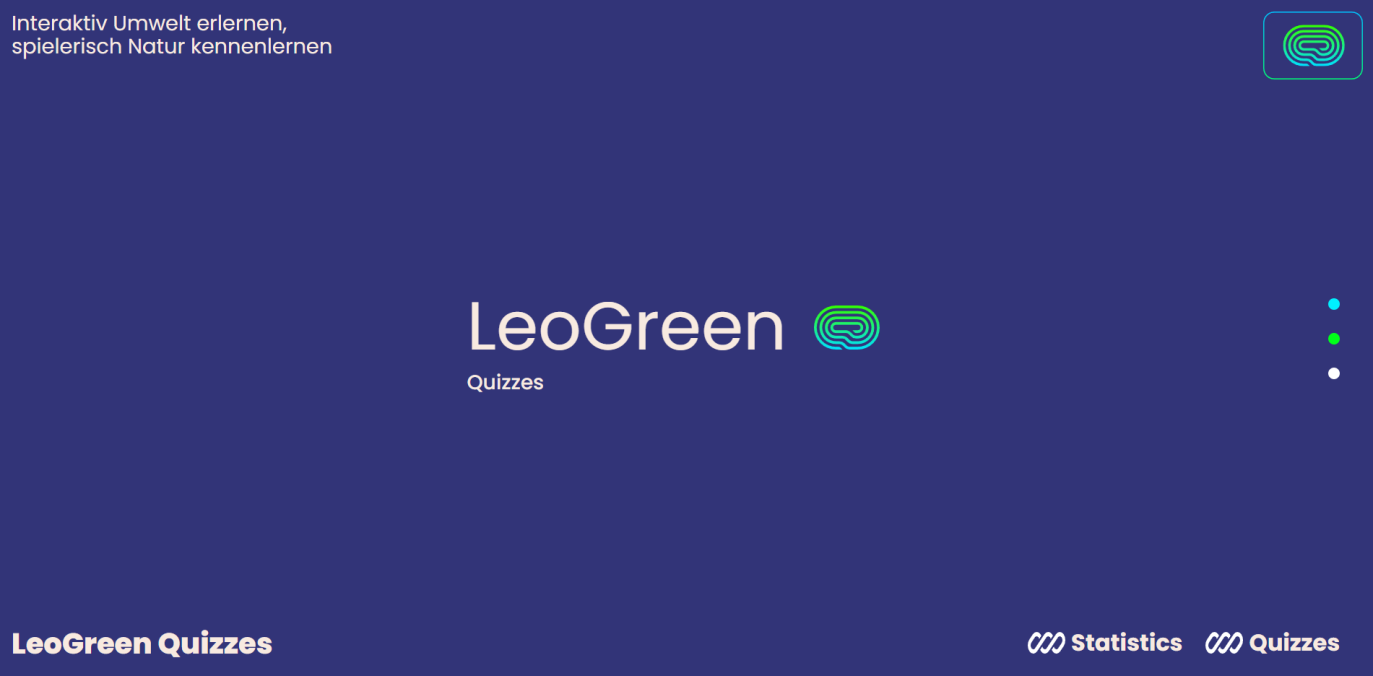
\includegraphics[scale=0.3]{pics/image.png}
    \caption{Startseite}
    \label{fig:impl:img1}
\end{figure}
\begin{figure}
    \centering
    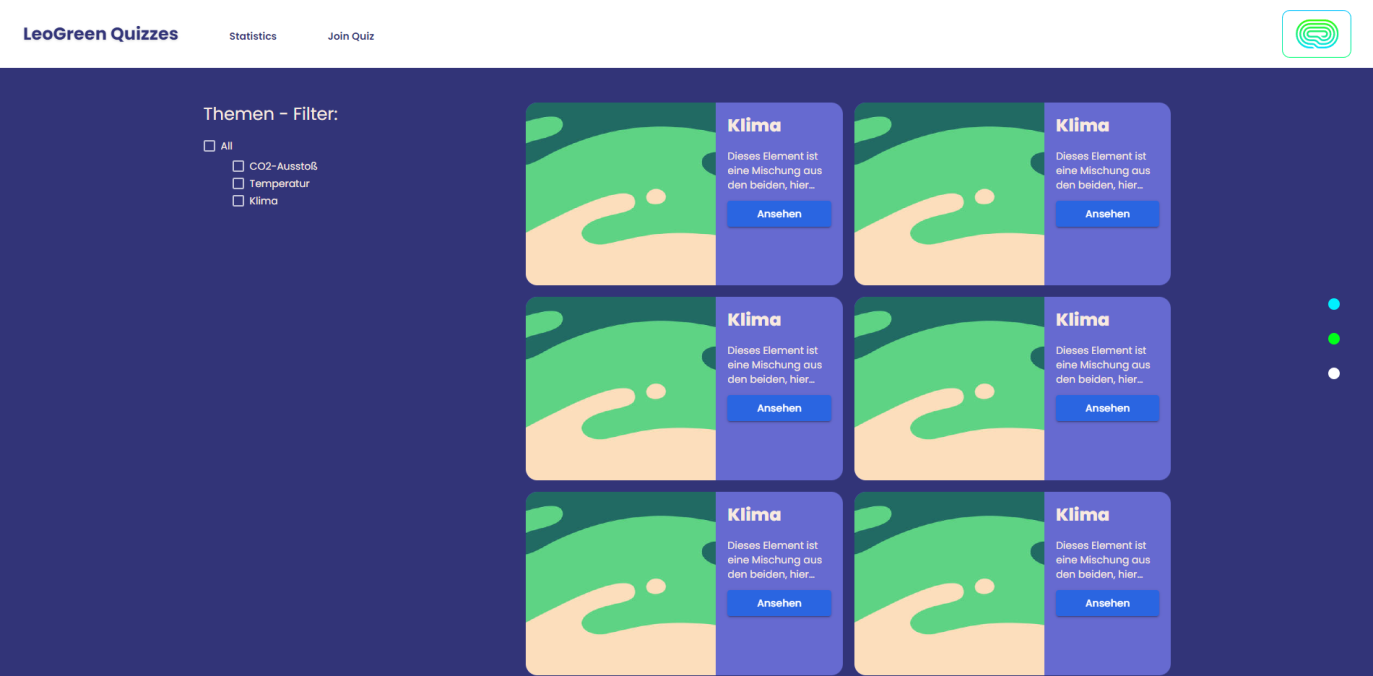
\includegraphics[scale=0.3]{pics/image (1).png}
    \caption{Lesson Übersicht}
    \label{fig:impl:img2}
\end{figure}
\begin{figure}
    \centering
    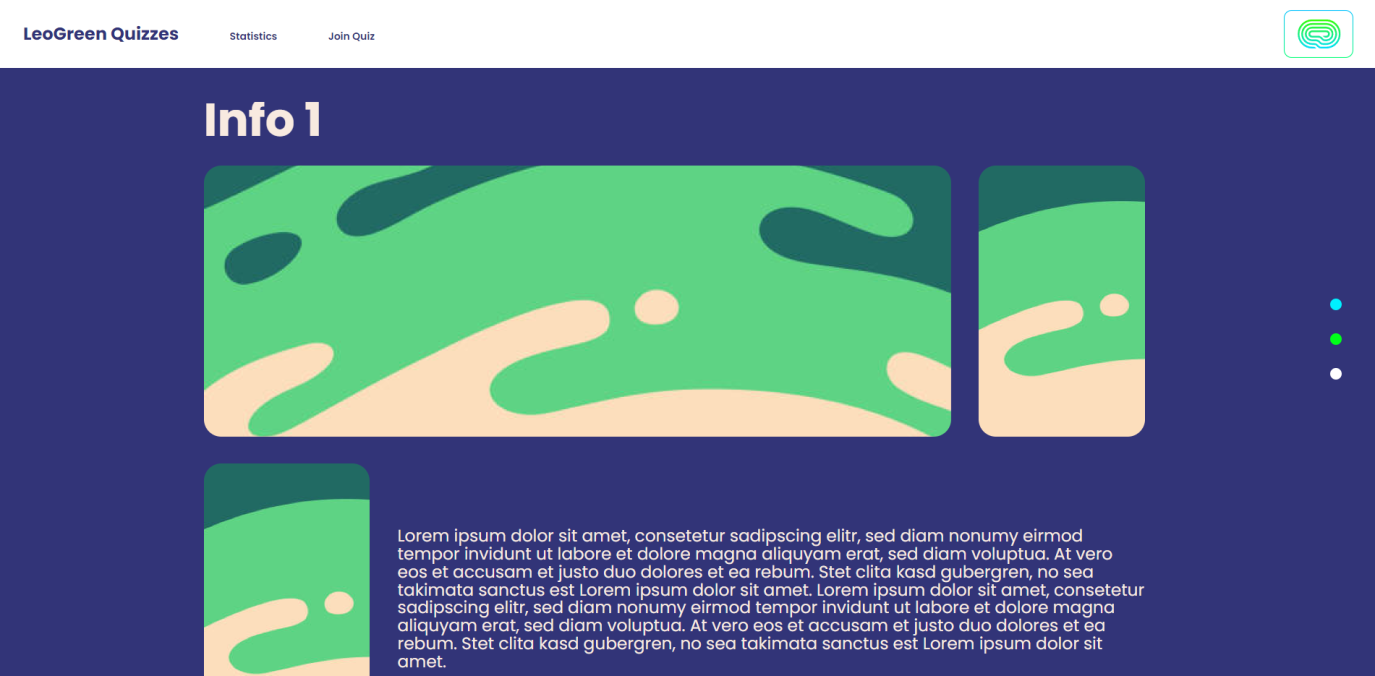
\includegraphics[scale=0.3]{pics/image (2).png}
    \caption{Lesson im Detail}
    \label{fig:impl:img3}
\end{figure}
\begin{figure}
    \centering
    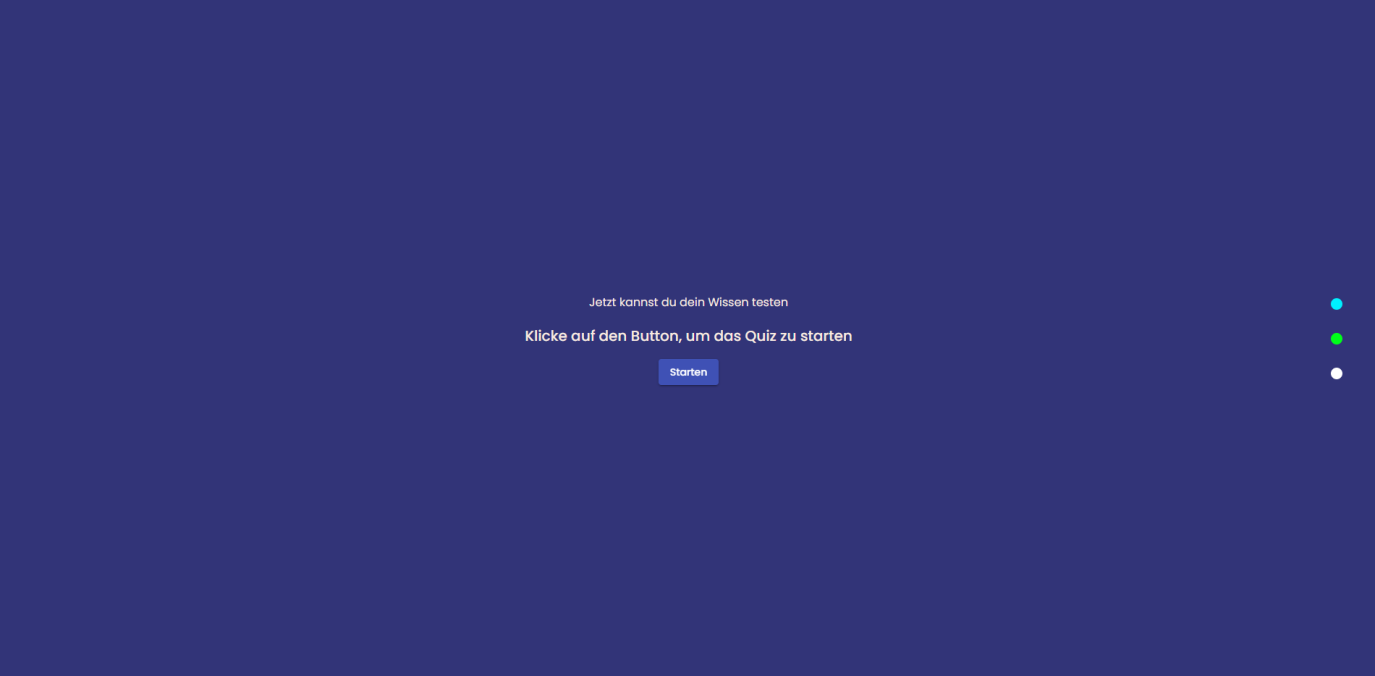
\includegraphics[scale=0.3]{pics/image (3).png}
    \caption{Starte ein Quiz}
    \label{fig:impl:img4}
\end{figure}
\begin{figure}
    \centering
    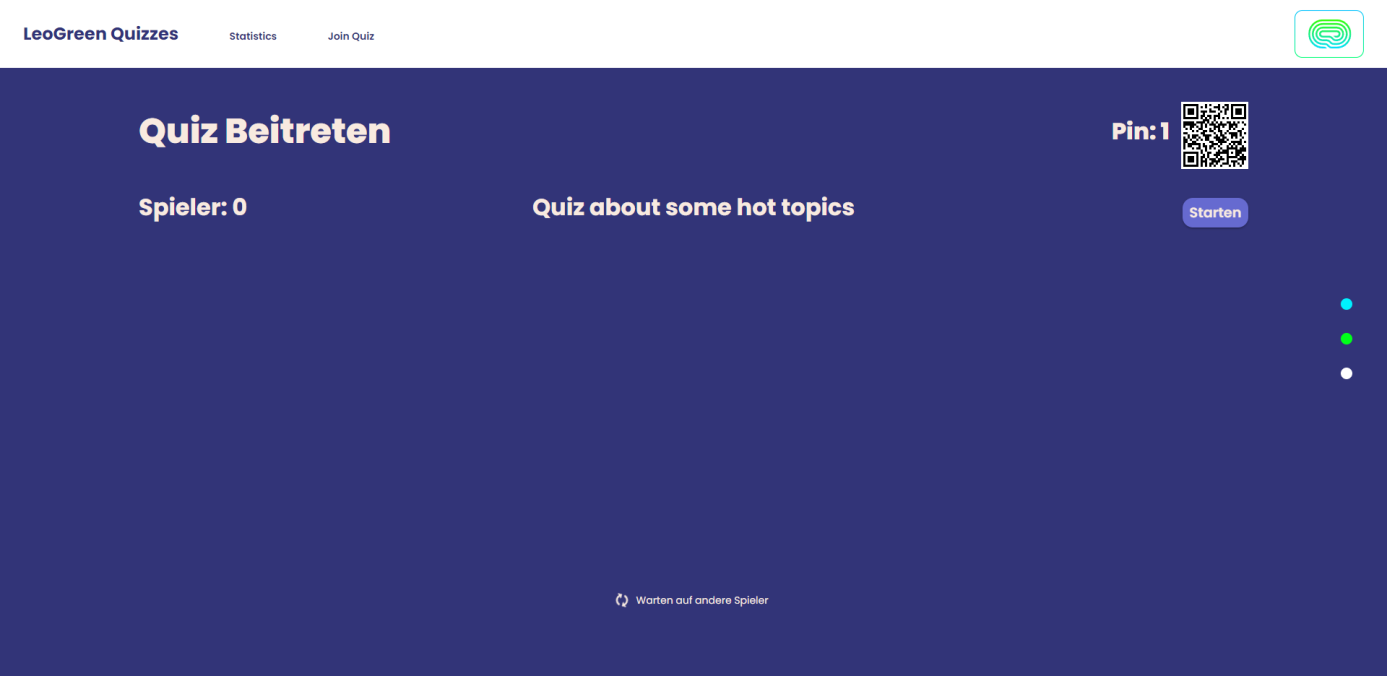
\includegraphics[scale=0.3]{pics/image (4).png}
    \caption{Warte auf Spieler}
    \label{fig:impl:img5}
\end{figure}
\begin{figure}
    \centering
    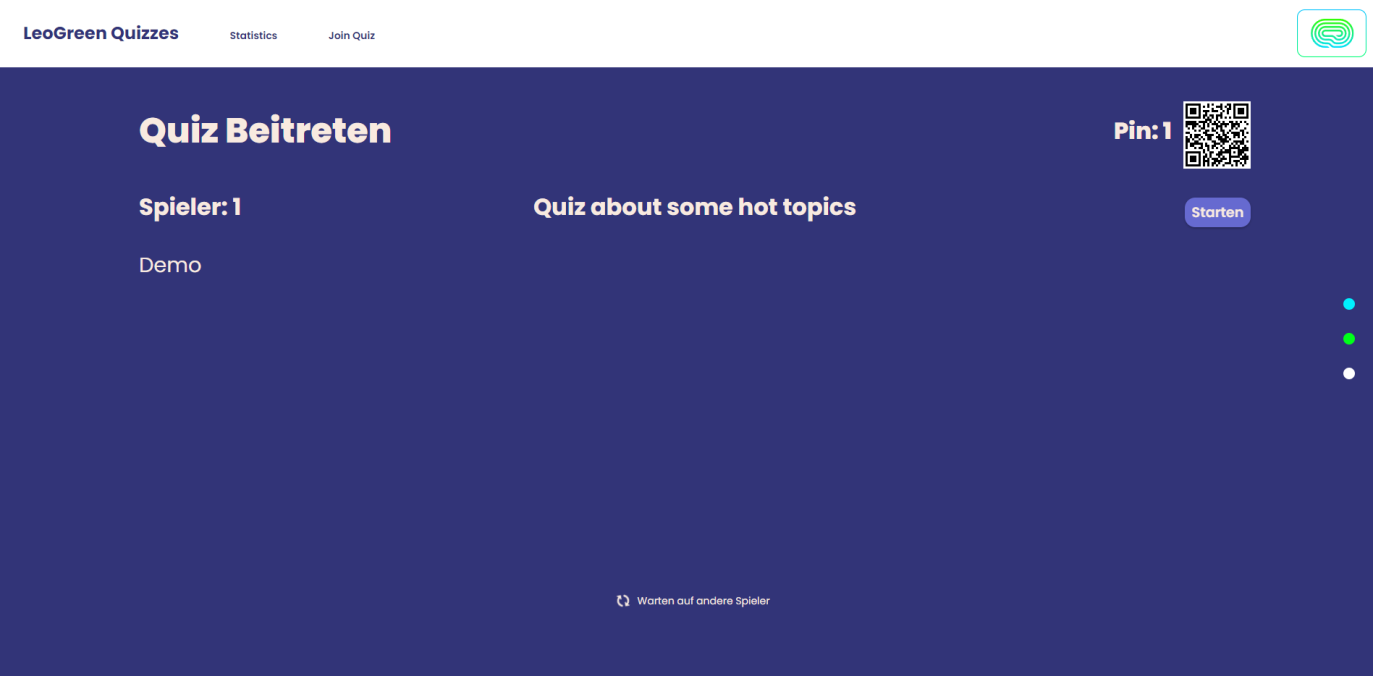
\includegraphics[scale=0.3]{pics/image (5).png}
    \caption{Der Player (Demo) ist gejoined}
    \label{fig:impl:img6}
\end{figure}
\begin{figure}
    \centering
    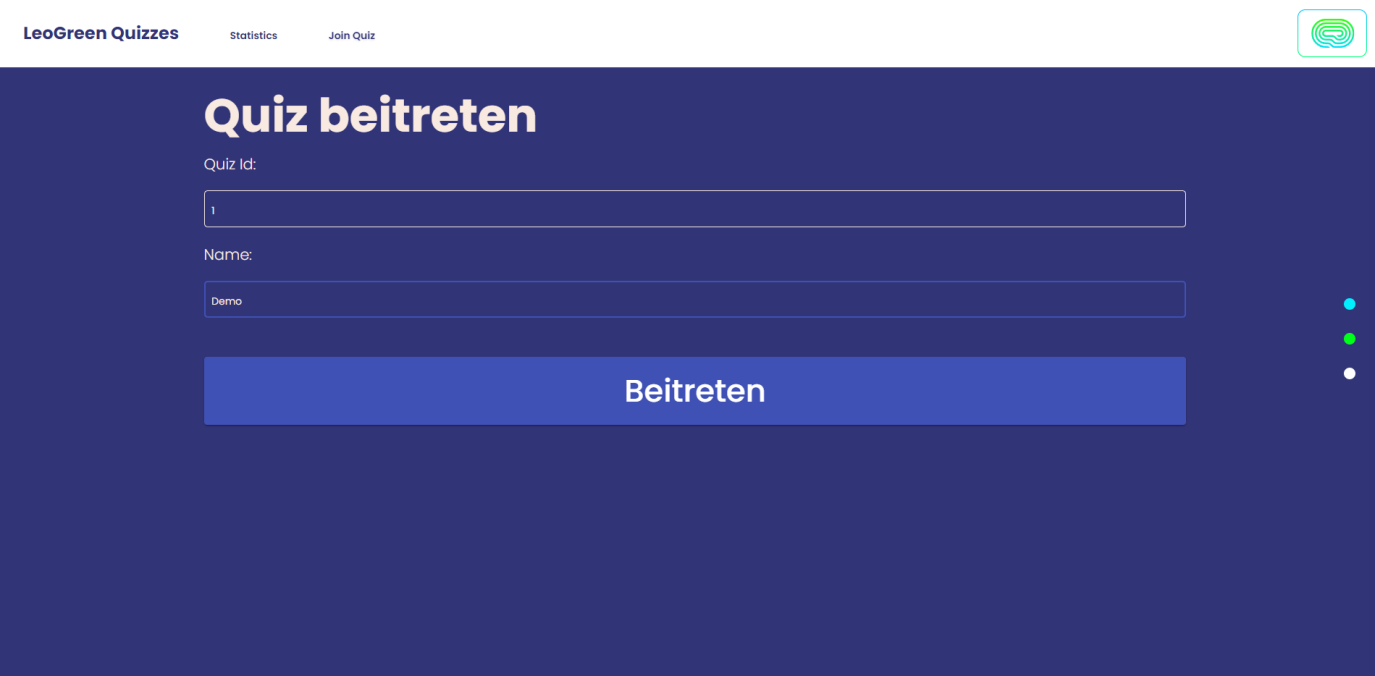
\includegraphics[scale=0.3]{pics/image (6).png}
    \caption{Trete einem Quiz bei (Schüleransicht)}
    \label{fig:impl:img7}
\end{figure}
\begin{figure}
    \centering
    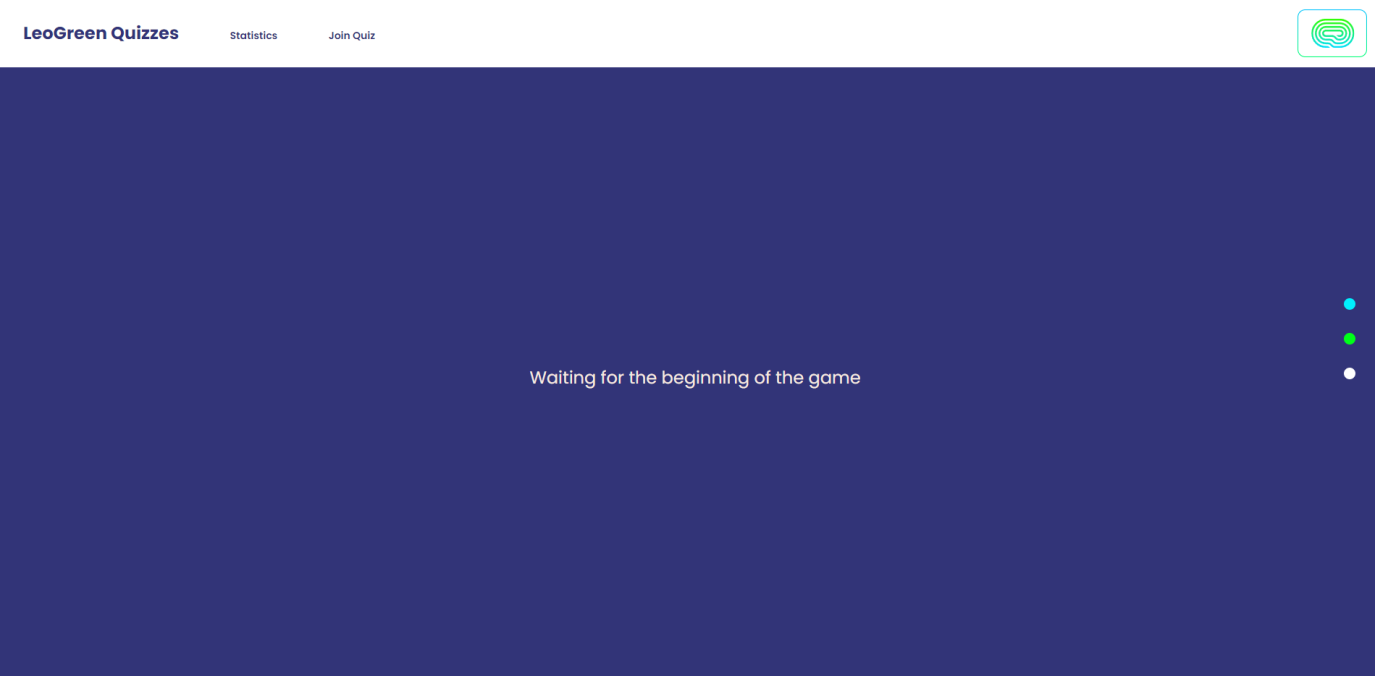
\includegraphics[scale=0.3]{pics/image (7).png}
    \caption{Auf den Start des Quizzes warten}
    \label{fig:impl:img8}
\end{figure}
\begin{figure}
    \centering
    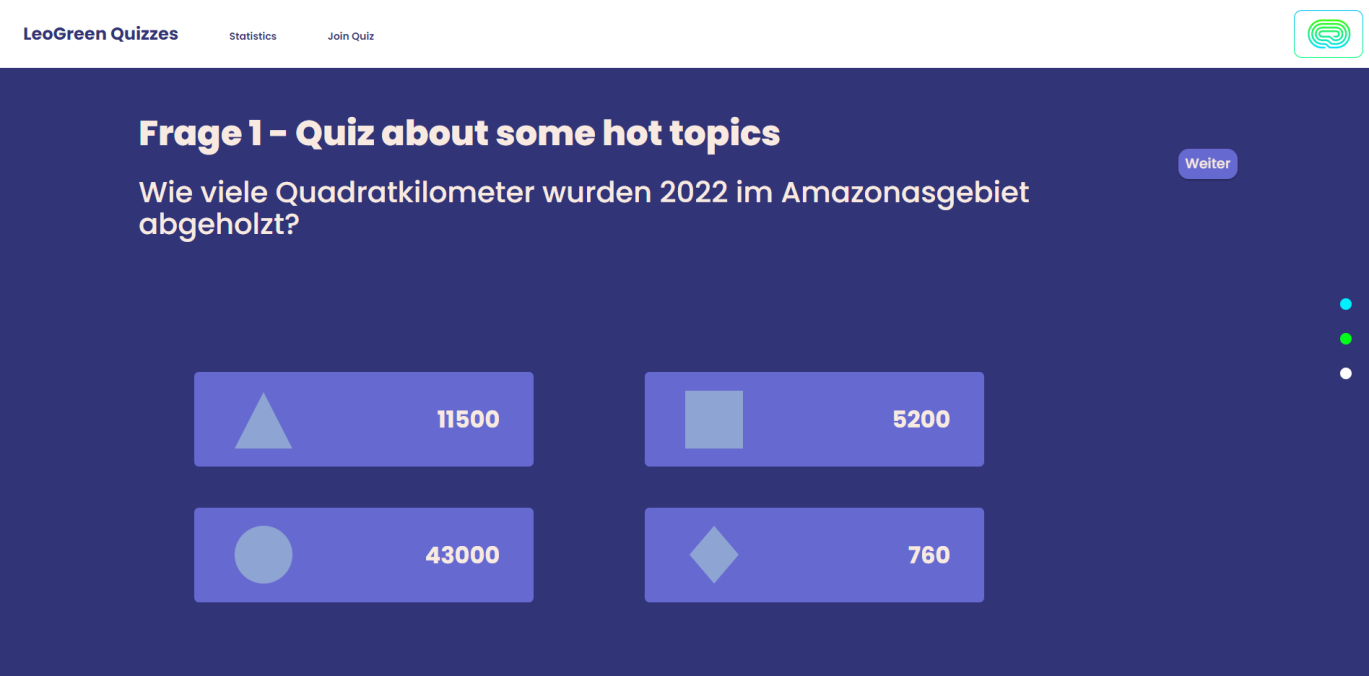
\includegraphics[scale=0.3]{pics/image (8).png}
    \caption{Ansicht der Fragen aus der Perspektive des Lehrers}
    \label{fig:impl:img9}
\end{figure}
\begin{figure}
    \centering
    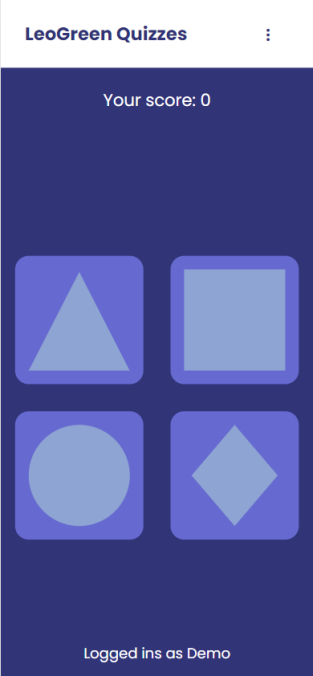
\includegraphics[scale=0.4]{pics/image (9).png}
    \caption{Mobile Ansicht der Schüler }
    \label{fig:impl:img10}
\end{figure}
\begin{figure}
    \centering
    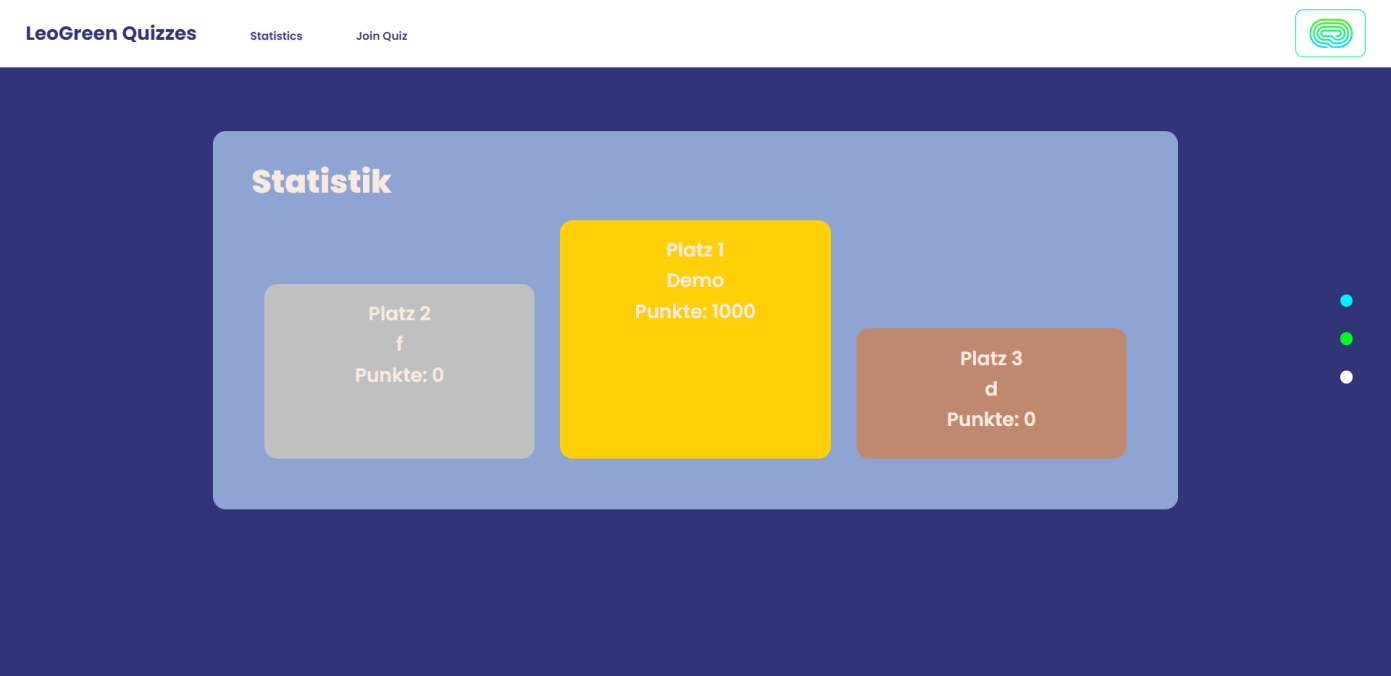
\includegraphics[scale=0.3]{pics/image (10).png}
    \caption{Die Besten Schüler aus einem Quiz, nach Punkten sortiert}
    \label{fig:impl:img11}
\end{figure}

Startseite von Leogreen \ref{fig:impl:img1}.

Übersicht der einzelnen Lessons \ref{fig:impl:img2}.

Inahlt einer Lesson, mit Bildern und Statistiken \ref{fig:impl:img3}.

Unter einer Lesson, der Abschnitt, um ein Quiz zu starten \ref{fig:impl:img4}.

Übersicht der schüler, welcher schon einem Quiz beigetreten sind \ref{fig:impl:img5}.

Demo 1 joined the game \ref{fig:impl:img6}.

Ansicht der Schüler, wenn sie ein Quiz beitreten möchten \ref{fig:impl:img7}.

Ladescreen, wenn man einem Quiz beigetreten ist, es aber noch nicht gestartet wurde \ref{fig:impl:img8}.

Ansicht der Lehrer, welche die Fragen dann über einen Beamer oder ein Display den Schülern zeigen \ref{fig:impl:img9}.

Smartphone ansicht der Antwortmöglichkeiten. \ref{fig:impl:img10}.

Übersicht der besten 3 Spieler einens Quizzes \ref{fig:impl:img11}.



